\documentclass[handout,t,compress]{beamer}
\usetheme{Singapore}

\sloppy
%\usepackage[scaled]{helvet}
%\usepackage{eulervm}

\usepackage{fp-eval}
\usepackage{hyperref}
\usepackage{fancyvrb}
%\usepackage{pstricks,pst-node,pst-tree,pst-plot,pst-3dplot,multido}
\usepackage{graphicx}
\usepackage{multicol}

\usepackage{alltt}

\newcommand{\bi}{\begin{itemize}}
\newcommand{\li}{\item}
\newcommand{\ei}{\end{itemize}}

\newcommand{\sect}[1]{\begin{frame}[fragile]{#1}}

\newcommand{\bbnf}{\begin{center}\begin{tabular}{rcl}}
\newcommand{\bnf}[2]{#1 & ::= & #2 \\}
\newcommand{\ebnf}{\end{tabular}\end{center}}

\newcommand{\myskip}{\vspace{-1em}\hrulefill}
\newcommand{\myrule}[1]{\vspace{-1ex}\centerline{\rule{#1cm}{1pt}}}
\newcommand{\myline}[1]{\centerline{#1}}
\newcommand{\bkt}[1]{\ensuremath{\langle\mbox{#1}\rangle}}
\newcommand{\br}{\mbox{~}|\mbox{~}}

\definecolor{orange}{rgb}{1,.5,0}
\definecolor{pink}{rgb}{1,.75,.75}
\definecolor{ltblue}{rgb}{.75,.75,1}

\newcommand{\be}{\begin{eqnarray*}}
\newcommand{\ee}{\end{eqnarray*}}

\newcommand{\grph}[2]{
\begin{columns}
\column{0.01\textwidth}
\column{0.6\textwidth}
\begin{pspicture}[showgrid=#1](-2,-2)(5,5)
#2
\end{pspicture}
}

\AtBeginSection[]
{
\sect{Outline}
\tableofcontents[currentsection]
\end{frame}
}

\title{Finite State Machines}
\author{CSCI 321}
\institute{WWU}

\begin{document}



\sect{~}
\titlepage
\end{frame}

\sect{Simple State Machine}
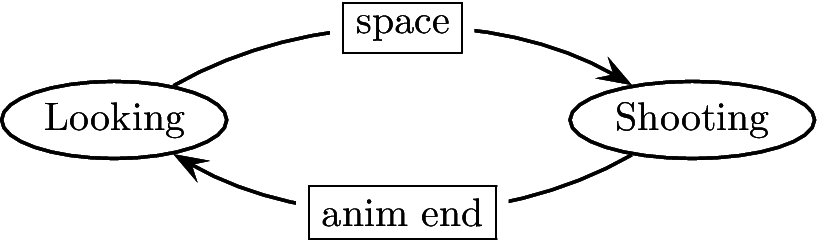
\includegraphics[scale=0.33]{simplestatemachine.png}
\end{frame}

\sect{More Complex State Machine}
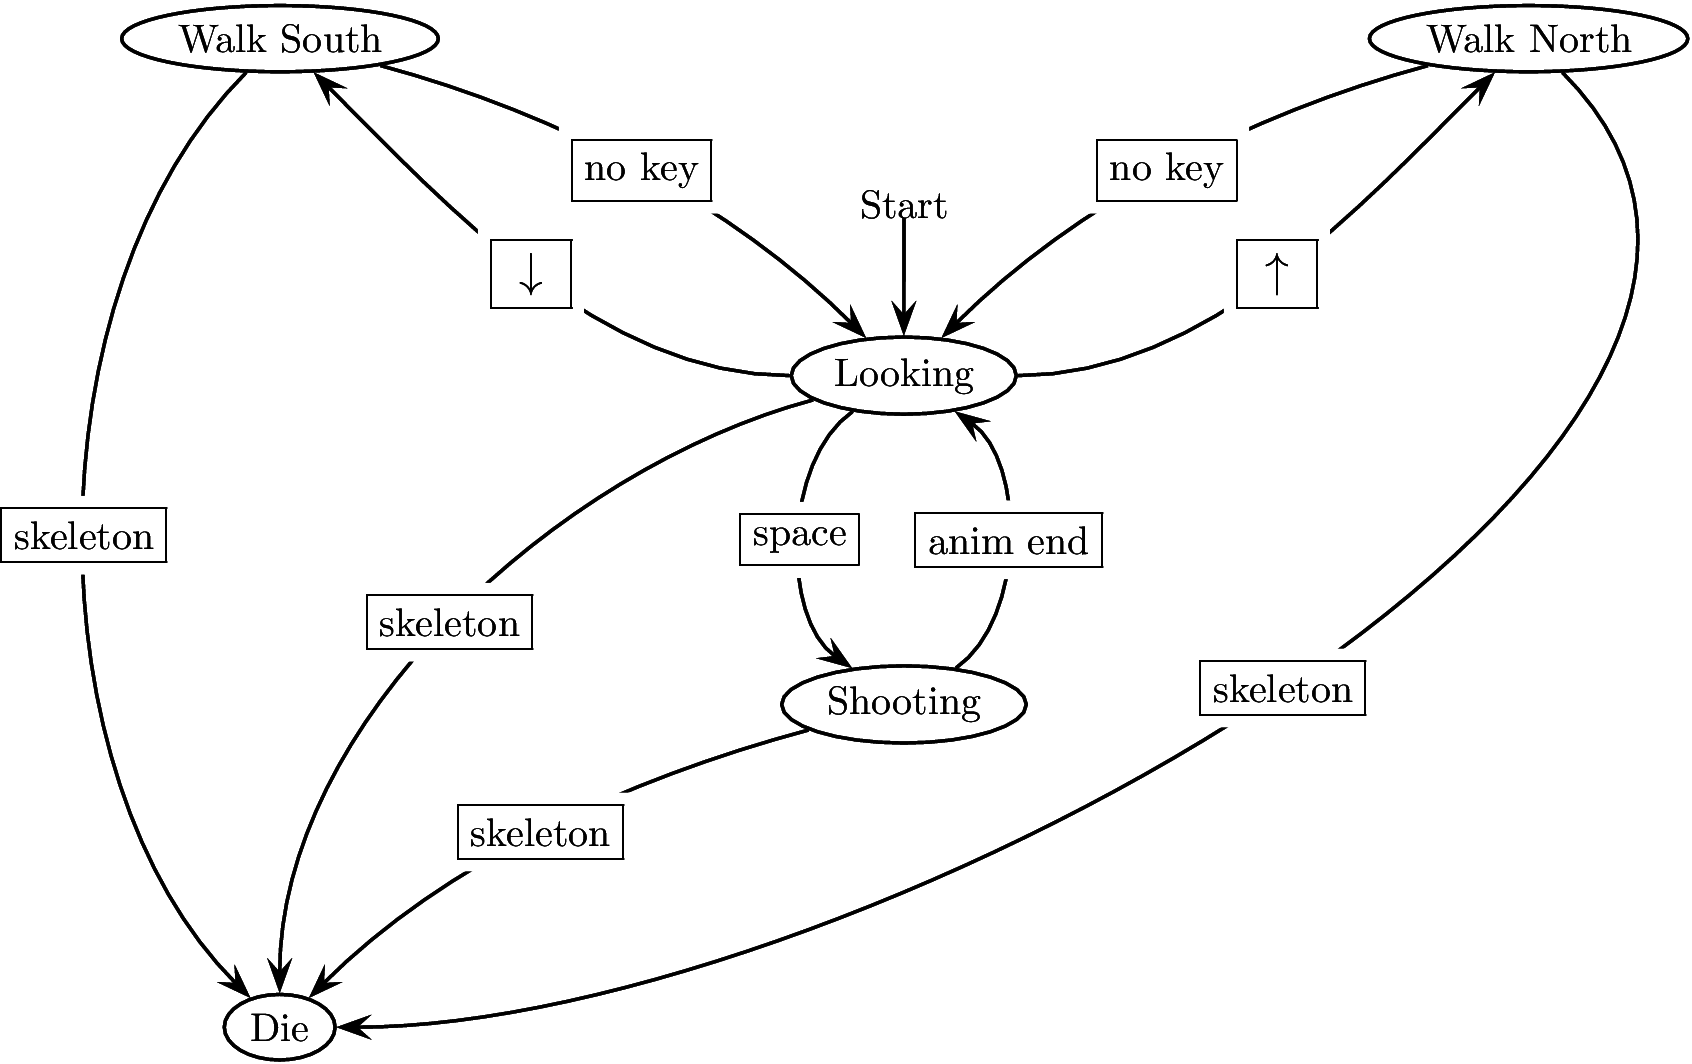
\includegraphics[scale=0.18]{stanstatemachine.png}
\end{frame}

\sect{Advantages of State Machines}
\bi
\li Quick and simple to code
\li Easy to debug
\li Little computational overhead
\li Intuitive and easy to understand
\li Flexible
\bi
\li Add new states
\li Add new rules
\li Add sub-machines and super-machines
\ei
\ei
\end{frame}

\sect{FSM implementation 1.0:  If-then statements}
%\begin{multicols}{2}
\scriptsize
\begin{Verbatim}
case CurrentState:
  EvadeEnemy:
    ...
    if Safe():
      ChangeState(Patrol)
    ...
  Patrol:
    ...
    if Threatened():
      if StrongerThanEnemy():
        ChangeState(Attack)
      else:
        ChangeState(Runaway)
    ...
  Attack:
    ...
    if not(StrongerThanEnemy()):
      ChangeState(Runaway)
    ...
  Runaway:
    ...  
\end{Verbatim}
%\end{multicols}
\end{frame}

\sect{FSM Implementation 2.0: Transition Tables}
\footnotesize
\begin{tabular}{|l|l|l|}\hline
{\bf Current State} & {\bf Condition} & {\bf State Transition} \\\hline
Runaway & Safe & Patrol\\
Attack & WeakerThanEnemy & Runaway\\
Patrol & Threatened AND StrongerThanEnemy & Attack\\
Patrol & Threatened AND WeakerThanEnemy & Runaway\\\hline
\end{tabular}
\end{frame}

\sect{FSM Implementation 3.0: Embedded Rules}
\begin{itemize}
\item Embed transitions in the states themselves.
\item There is no master control or code.
\item Easily extensible--only affected states need be modified.
\item {\bf State Design Pattern}
\end{itemize}
\end{frame}

\sect{Miner Bob's State Diagram}

\bigskip

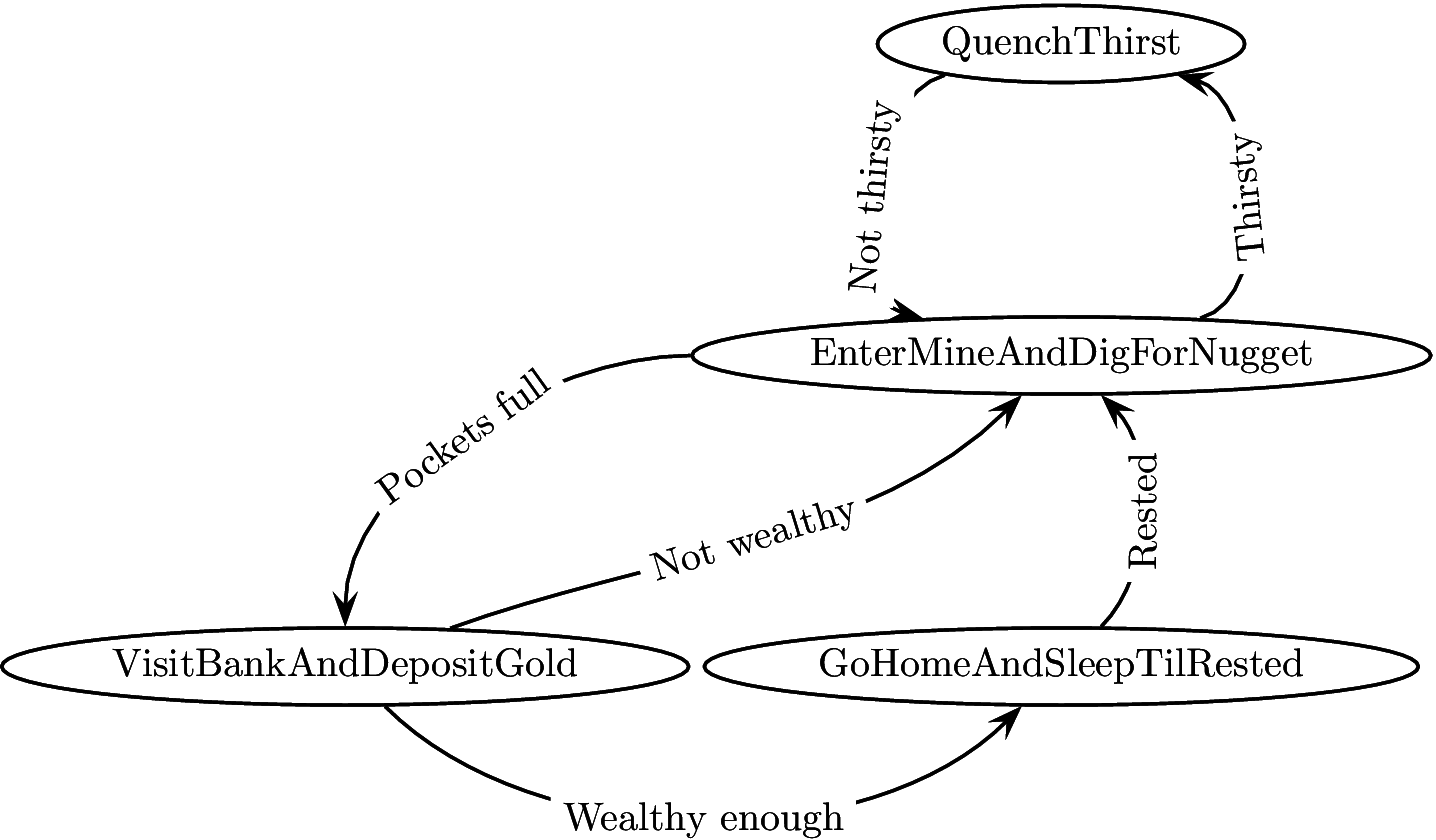
\includegraphics[width=\textwidth]{figure2-2.png}
\end{frame}

\sect{Global States and State Blips}

\bi
\li Some things may happen at any time, no matter what state you're in.
\bi
\li E.g., going to the bathroom.
\li Use a {\bf Global State} for these.
\li Global state updated every clock tick, in addition to the current
state. 
\ei

\li Need to remember what you were doing previously.
\bi
\li Use a {\bf Blip State} for these.
\li Push current state in to a previous state pointer.
\li Should use a stack, but sometimes not necessary.
\ei
\li See Figure 2.4
\ei

\end{frame}


\sect{Elsa's State Diagram}

\bigskip

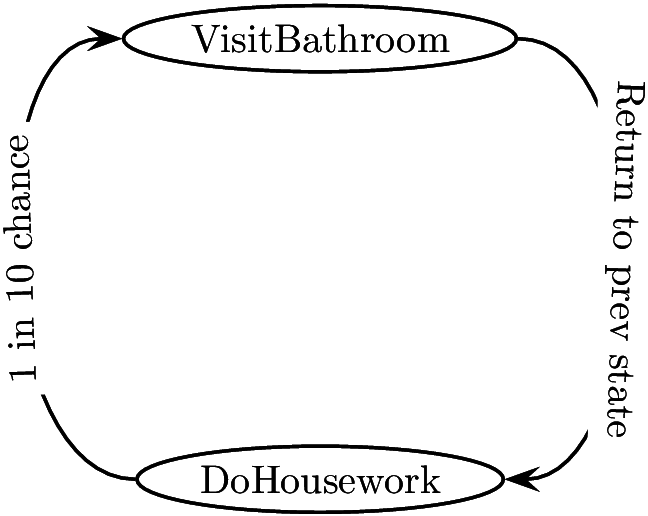
\includegraphics[width=0.5\textwidth]{figure2-5.png}
\end{frame} 

\sect{Messaging}
\bi
\li Events in one object can trigger events in other objects.
\li Intuitive way to design this is a {\bf message} system.
\li {\tt Telegram} structure and {\tt MessageDispatcher} class.
\li Also uses an {\tt EntityManager} so that IDs can be mapped to
entities. 
\li Entities have {\tt HandleMessage} added.
\li States have {\tt OnMessage} added.
\bi
\li Returns a boolean so messages can be rerouted if necessary.
\ei
\li See Figure 2.7
\ei
\end{frame}

\sect{Elsa's State Diagram with Messaging}

\bigskip

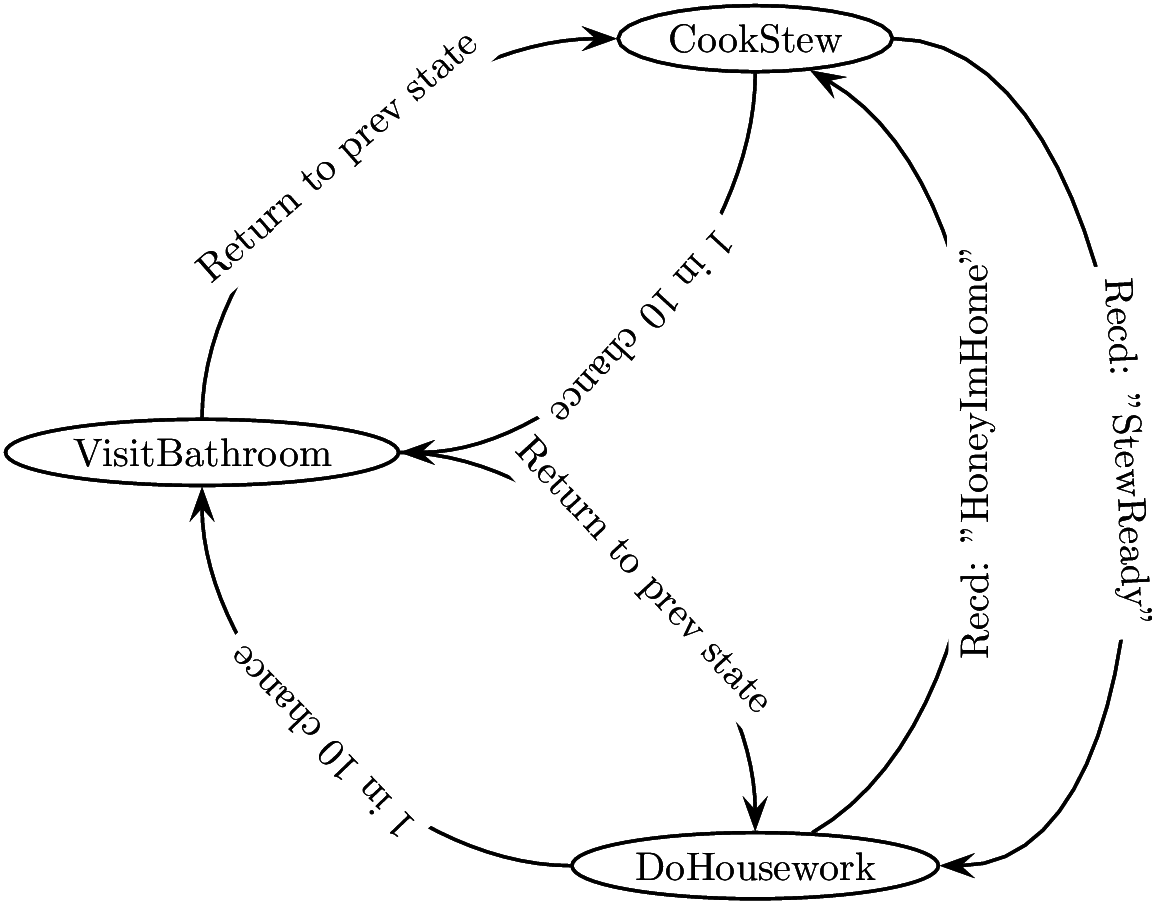
\includegraphics[width=0.75\textwidth]{figure2-6.png}
\end{frame}

\sect{Summing Up}

\bi
\li FSMs a good way to manage complex behavior.
\li Can use two FSMs in parallel, {\em e.g.}:
  \bi
  \li One for movement
  \li One for weapon selection, aiming, firing
  \ei
\li Can use hierarchical FSMs:
 one state machine inside the state of another, {\em e.g.}:
  \bi
  \li High level states:  {\bf Explore}, {\bf Combat}, {\bf Patrol}
  \li Low level states inside Combat:
  \bi \li Dodge \li ChaseEnemy \li Shoot \ei
  \ei
\ei

\end{frame}

\end{document}
